\section{外显子组测序}
\subsection{简介}
\begin{frame}
  \frametitle{外显子组测序 | 简介 | \textcolor{red}{Exome}}
  The exome is the part of the genome formed by exons, the sequences which when transcribed remain within the mature RNA after introns are removed by RNA splicing. It consists of all DNA that is transcribed into mature RNA in cells of any type as distinct from the transcriptome, which is the RNA that has been transcribed only in a specific cell population.
  \begin{figure}
    \centering
    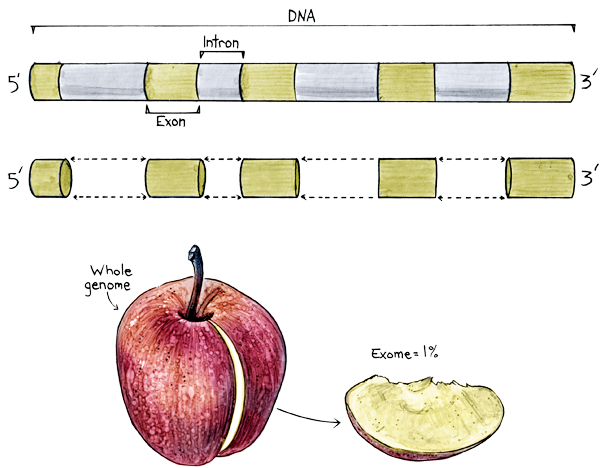
\includegraphics[width=0.5\textwidth]{c2.genomics/exome.01.png}
  \end{figure}
\end{frame}

\begin{frame}
  \frametitle{外显子组测序 | 简介 | \textcolor{red}{Exome}}
  The exome of the human genome consists of roughly 180,000 exons constituting about 1\% of the total genome, or about 30 megabases of DNA. Though comprising a very small fraction of the genome, mutations in the exome are thought to harbor 85\% of mutations that have a large effect on disease.
  \begin{figure}
    \centering
    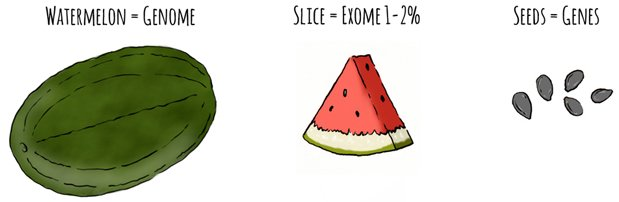
\includegraphics[width=0.8\textwidth]{c2.genomics/exome.02.jpg}
  \end{figure}
\end{frame}

\begin{frame}
  \frametitle{外显子组测序 | 简介 | Exome sequencing}
  \begin{block}{\textcolor{red}{WES}}
  Exome sequencing, also known as whole exome sequencing (WES or WXS), is a technique for sequencing all the expressed genes in a genome (known as the exome).
  \end{block}
  \pause
  \begin{block}{Projects}
    Examples of research projects using exome sequencing include:
    \begin{itemize}
      \item PGP (Personal Genome Project)
      \item RGI (Rare Genomics Institute)
      \item NIH-funded Exome Project
      \item NHGRI-funded Mendelian Exome Project
      \item NHLBI Grand Opportunity Exome Sequencing Project
      \item microarray-based Nimblegen SeqCap EZ Exome from Roche Applied Science
    \end{itemize}
  \end{block}
\end{frame}

\begin{frame}
  \frametitle{外显子组测序 | 简介 | Exome sequencing}
  Exome sequencing consists of first selecting only the subset of DNA that encodes proteins (known as exons) and then sequencing that DNA using any high-throughput DNA sequencing technology.\\
  \vspace{1em}
  Humans have about 180,000 exons, constituting about 1\% of the human genome, or approximately 30 million base pairs.\\
  \vspace{1em}
  The goal of this approach is to identify genetic variation that is responsible for both Mendelian and common diseases such as Miller syndrome and Alzheimer's disease without the high costs associated with whole-genome sequencing.\\
  \vspace{1em}
  Exome sequencing has proved to be an efficient strategy to determine the genetic basis of more than two dozen Mendelian or single gene disorders.
\end{frame}

\begin{frame}
  \frametitle{外显子组测序 | 简介 | Exome sequencing}
  \begin{figure}
    \centering
    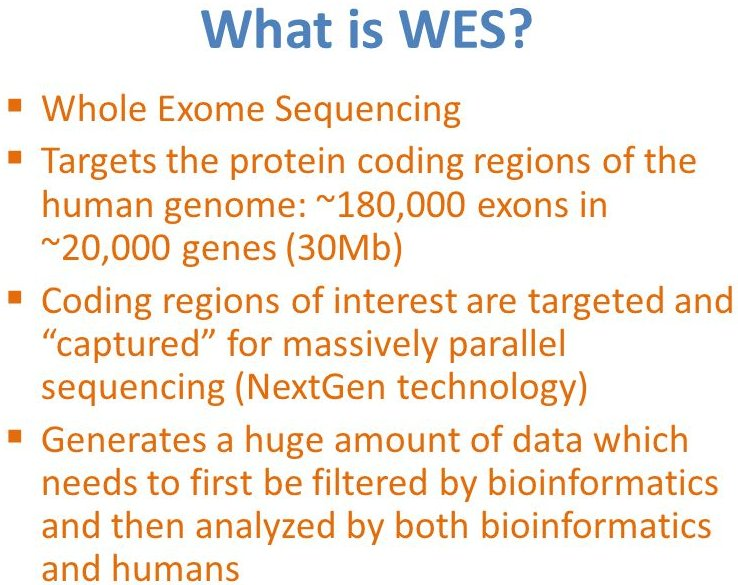
\includegraphics[width=0.8\textwidth]{c2.genomics/exome.wes.01.jpg}
  \end{figure}
\end{frame}

\begin{frame}
  \frametitle{外显子组测序 | 简介 | Exome sequencing}
  \begin{figure}
    \centering
    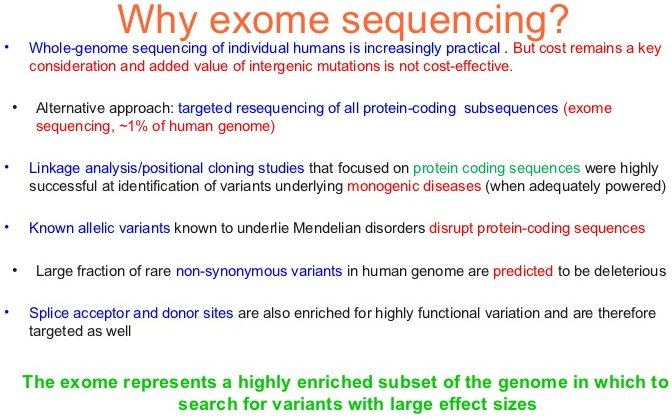
\includegraphics[width=0.9\textwidth]{c2.genomics/exome.wes.02.jpg}
  \end{figure}
\end{frame}

\begin{frame}
  \frametitle{外显子组测序 | 简介 | \textcolor{red}{Exome sequencing}}
  \begin{figure}
    \centering
    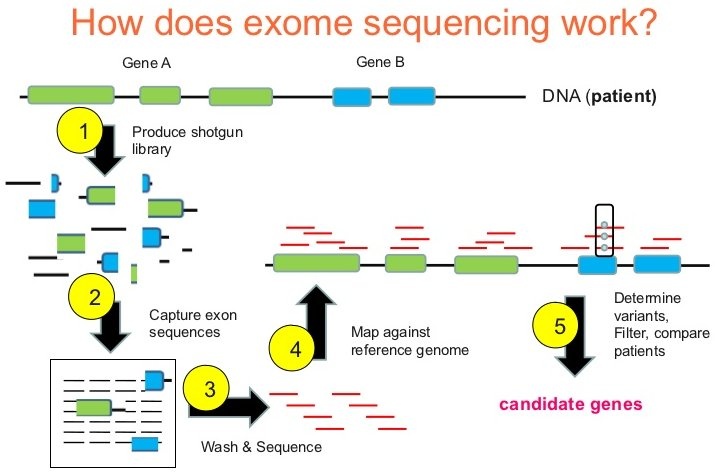
\includegraphics[width=0.9\textwidth]{c2.genomics/exome.wes.03.jpg}
  \end{figure}
\end{frame}

\begin{frame}
  \frametitle{外显子组测序 | 简介 | Exome sequencing}
  \begin{figure}
    \centering
    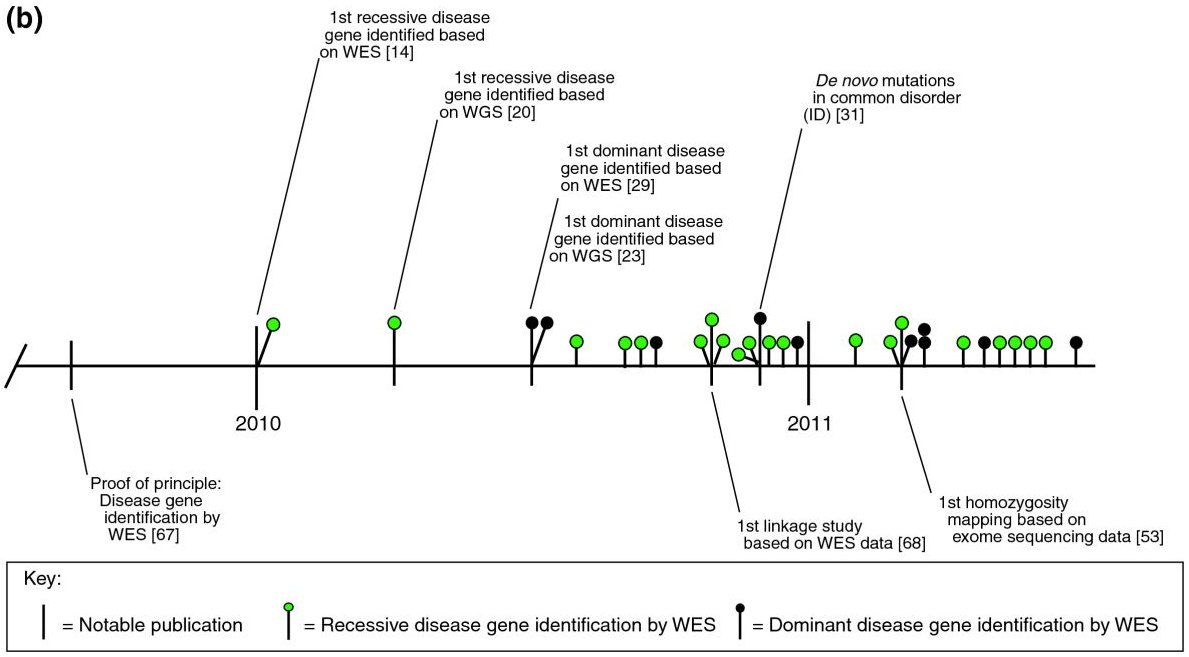
\includegraphics[width=0.9\textwidth]{c2.genomics/exome.wes.04.jpg}
  \end{figure}
\end{frame}

\begin{frame}
  \frametitle{外显子组测序 | 简介 | Exome sequencing | WGS}
  \begin{block}{WGS}
    Whole genome sequencing (also known as WGS, full genome sequencing, complete genome sequencing, or entire genome sequencing) is a laboratory process that determines the complete DNA sequence of an organism's genome at a single time.\\
    \vspace{1em}
    This entails sequencing all of an organism's chromosomal DNA as well as DNA contained in the mitochondria and, for plants, in the chloroplast.
  \end{block}
\end{frame}

\begin{frame}
  \frametitle{外显子组测序 | 简介 | Exome sequencing | WGS}
  \begin{figure}
    \centering
    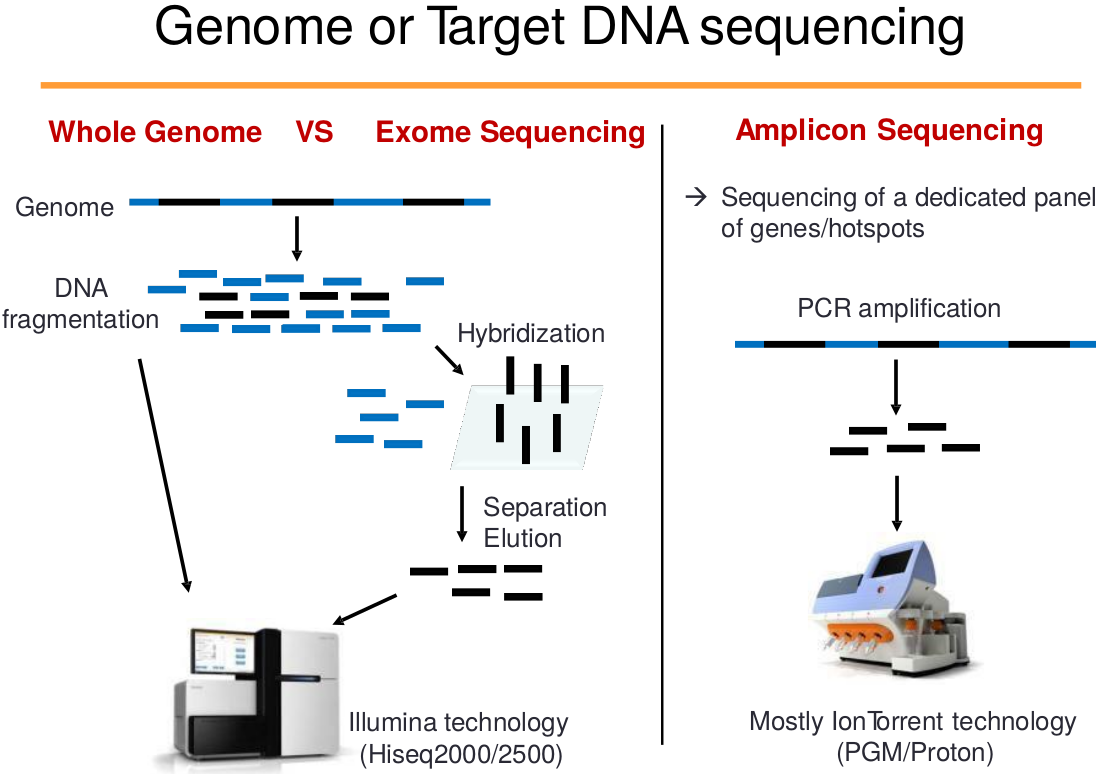
\includegraphics[width=0.9\textwidth]{c2.genomics/exome.wgs.01.png}
  \end{figure}
\end{frame}

\begin{frame}
  \frametitle{外显子组测序 | 简介 | Exome sequencing | Comparison}
  \begin{block}{SNP array}
    \begin{itemize}
      \item require hybridization probes of a known sequence
      \item can only detect shared genetic variants that are common to many individuals in the wider population
    \end{itemize}
  \end{block}
  \pause
  \begin{block}{whole genome sequencing}
    high costs and time associated with sequencing large numbers of genomes
    %\verb|$_$| All money money go my home \verb|$_$|
  \end{block}
\end{frame}

\begin{frame}
  \frametitle{外显子组测序 | 简介 | Exome sequencing | Comparison}
  \begin{block}{Exome sequencing}
    \begin{itemize}
      \item the most efficient way to identify the genetic variants in all of an individual's genes $\Rightarrow$ especially effective in the study of rare Mendelian diseases
      \item severe disease causing variants are much more likely (but by no means exclusively) to be in the protein coding sequence $\Rightarrow$ focusing on this 1\% costs far less than whole genome sequencing but still produces a high yield of relevant variants
      \item both to find mutations in genes already known to cause disease as well as to identify novel genes by comparing exomes from patients with similar features
    \end{itemize}
  \end{block}
\end{frame}

\begin{frame}
  \frametitle{外显子组测序 | 简介 | Exome sequencing | Technique}
  \begin{block}{Techiniques}
    \begin{itemize}
      \item Target-enrichment strategies
      \item PCR
      \item Molecular inversion probes (MIP)
      \item Hybrid capture
      \item In-solution capture
      \item Sequencing
    \end{itemize}
  \end{block}
\end{frame}

\begin{frame}
  \frametitle{外显子组测序 | 简介 | Exome sequencing | Technique}
  \begin{block}{Target-enrichment strategies}
    Target-enrichment methods allow one to selectively capture genomic regions of interest from a DNA sample prior to sequencing. Several target-enrichment strategies have been developed since the original description of the direct genomic selection (DGS) method by the Lovett group in 2005.
  \end{block}
\end{frame}

\begin{frame}
  \frametitle{外显子组测序 | 简介 | Exome sequencing | Technique}
  \begin{block}{PCR}
    Polymerase chain reaction (PCR) is technology to amplify specific DNA sequences. It uses a single stranded piece of DNA as a start for DNA amplification. Uniplex PCR uses only one starting point (primer) for amplification and multiplex PCR uses multiple primers. This way multiple genes can be targeted simultaneously.
  \end{block}
\end{frame}

\begin{frame}
  \frametitle{外显子组测序 | 简介 | Exome sequencing | Technique}
  \begin{block}{Molecular inversion probes (MIP)}
    Molecular inversion probe uses probes of single stranded DNA oligonucleotides flanked by target-specific ends. The gaps between the flanking sequences are filled and ligated to form a circular DNA fragment. Probes that did not undergo reaction remain linear and are removed using exonucleases. This is an enzymatic technique that targets the amplification of genomic regions by multiplexing based on target circularization.
  \end{block}
  \begin{figure}
    \centering
    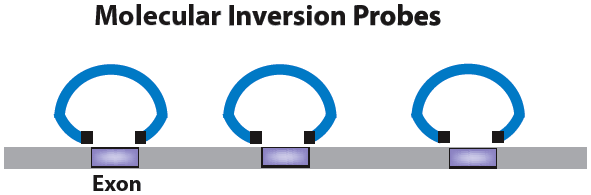
\includegraphics[width=0.7\textwidth]{c2.genomics/exome.mip.01.png}
  \end{figure}
\end{frame}

\begin{frame}
  \frametitle{外显子组测序 | 简介 | Exome sequencing | Technique}
  \begin{block}{Hybrid capture}
    Microarrays contain single-stranded oligonucleotides with sequences from the human genome to tile the region of interest fixed to the surface. Genomic DNA is sheared to form double-stranded fragments. The fragments undergo end-repair to produce blunt ends and adaptors with universal priming sequences are added. These fragments are hybridized to oligos on the microarray. Unhybridized fragments are washed away and the desired fragments are eluted. The fragments are then amplified using PCR.
  \end{block}
\end{frame}

\begin{frame}
  \frametitle{外显子组测序 | 简介 | Exome sequencing | Technique}
  \begin{block}{In-solution capture}
 To capture genomic regions of interest using in-solution capture, a pool of custom oligonucleotides (probes) is synthesized and hybridized in solution to a fragmented genomic DNA sample. The probes (labeled with beads) selectively hybridize to the genomic regions of interest after which the beads (now including the DNA fragments of interest) can be pulled down and washed to clear excess material. The beads are then removed and the genomic fragments can be sequenced allowing for selective DNA sequencing of genomic regions (e.g., exons) of interest.\\
 \vspace{1em}
 This method was developed to improve on the hybridization capture target-enrichment method.
  \end{block}
\end{frame}

\begin{frame}
  \frametitle{外显子组测序 | 简介 | Exome sequencing | Technique}
  \begin{figure}
    \centering
    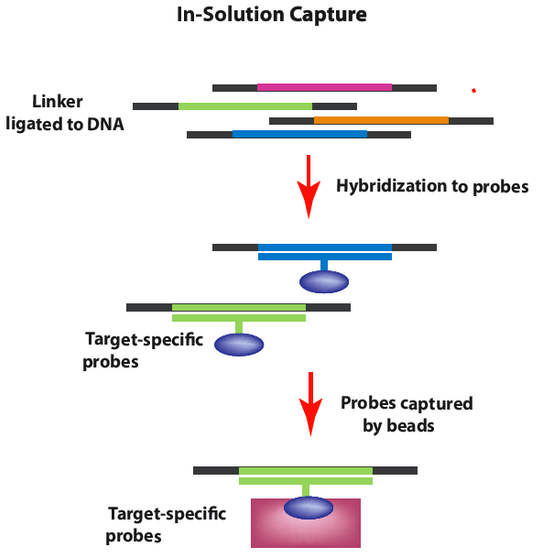
\includegraphics[width=0.6\textwidth]{c2.genomics/exome.isp.01.png}
  \end{figure}
\end{frame}

\begin{frame}
  \frametitle{外显子组测序 | 简介 | Exome sequencing | Technique}
  \begin{block}{Sequencing}
 There are several sequencing platforms available including the classical Sanger sequencing. Other platforms include the Roche 454 sequencer, the Illumina Genome Analyzer II and the Life Technologies SOLiD \& Ion Torrent all of which have been used for exome sequencing.
  \end{block}
\end{frame}

\begin{frame}
  \frametitle{外显子组测序 | 简介 | Exome sequencing | Significance}
  Exome sequencing has the potential to locate causative genes in complex diseases, which previously has not been possible due to limitations in traditional methods.\\
  \vspace{1em}
  Targeted capture and massively parallel sequencing represents a cost-effective, reproducible and robust strategy with high sensitivity and specificity to detect variants causing protein-coding changes in individual human genomes.
\end{frame}

\begin{frame}
  \frametitle{外显子组测序 | 简介 | Exome sequencing | Limitation}
  \begin{block}{Exome}
 Exome sequencing is only able to identify those variants found in the coding region of genes which affect protein function. It is not able to identify the structural and non-coding variants associated with the disease, which can be found using other methods such as whole genome sequencing. There remains 99\% of the human genome that is not covered using exome sequencing.
  \end{block}
\end{frame}

\begin{frame}
  \frametitle{外显子组测序 | 简介 | Exome sequencing | Limitation}
  \begin{block}{Statistical analysis}
    The statistical analysis of the large quantity of data generated from sequencing approaches is a challenge. False positive and false negative findings are associated with genomic resequencing approaches and is a critical issue. A few strategies have been developed to improve the quality of exome data such as:
    \begin{itemize}
      \item Comparing the genetic variants identified between sequencing and array-based genotyping
      \item Comparing the coding SNPs to a whole genome sequenced individual with the disorder
      \item Comparing the coding SNPs with Sanger sequencing of HapMap individuals
    \end{itemize}
  \end{block}
\end{frame}

\begin{frame}
  \frametitle{外显子组测序 | 简介 | Exome sequencing | \textcolor{red}{Application}}
  By using exome sequencing, fixed-cost studies can sequence samples to much higher depth than could be achieved with whole genome sequencing. This additional depth makes exome sequencing well suited to several applications that need reliable variant calls.
  \begin{itemize}
    \item Rare variant mapping in complex disorders
    \item Discovery of Mendelian disorders
    \item Clinical diagnostics
    \item Direct-to-consumer exome sequencing
  \end{itemize}
\end{frame}

\subsection{操作流程}
\begin{frame}
  \frametitle{外显子组测序 | 流程 | 实验}
  \begin{figure}
    \centering
    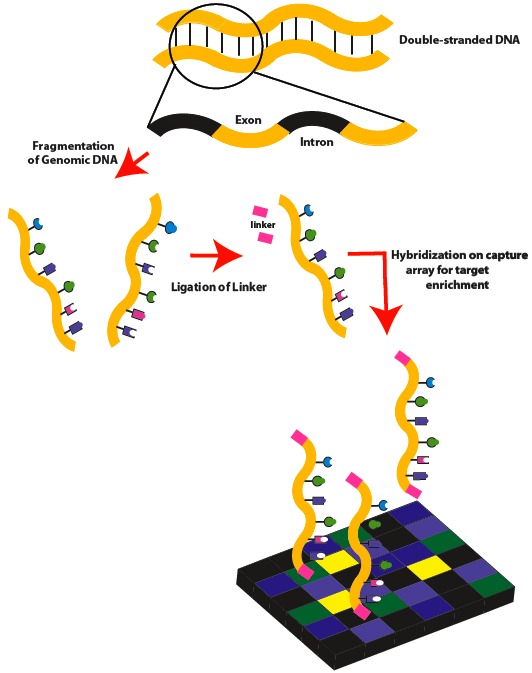
\includegraphics[width=0.5\textwidth]{c2.genomics/exome.exp.01.png}
  \end{figure}
\end{frame}

\begin{frame}
  \frametitle{外显子组测序 | 流程 | 实验}
  \begin{figure}
    \centering
    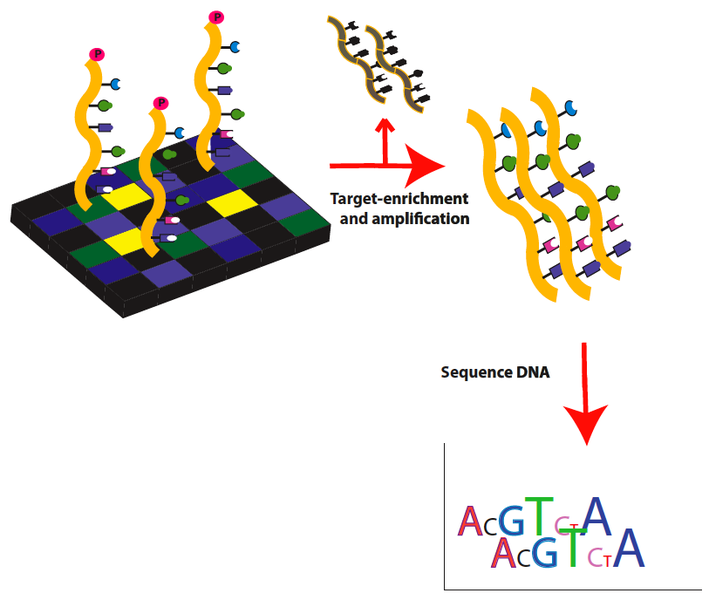
\includegraphics[width=0.7\textwidth]{c2.genomics/exome.exp.02.png}
  \end{figure}
\end{frame}

\begin{frame}
  \frametitle{外显子组测序 | 流程 | \textcolor{red}{实验}}
  \begin{figure}
    \centering
    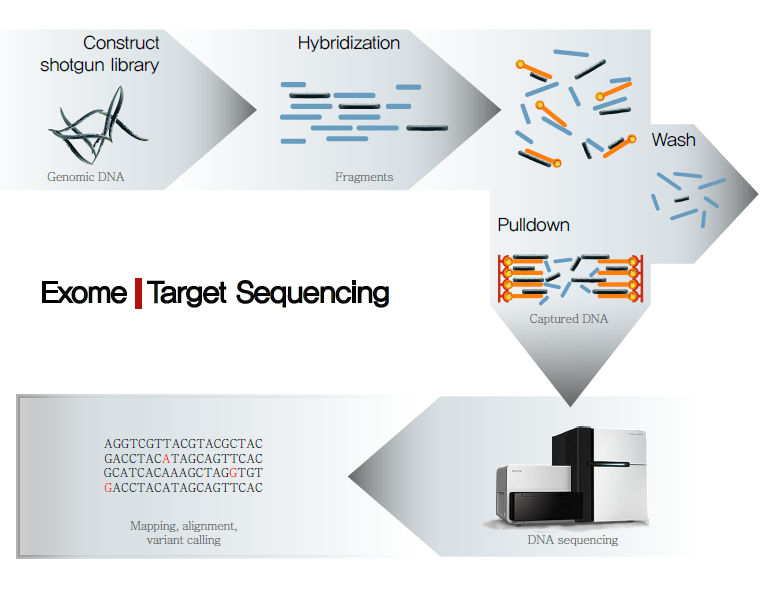
\includegraphics[width=0.85\textwidth]{c2.genomics/exome.exp.03.png}
  \end{figure}
\end{frame}

\begin{frame}
  \frametitle{外显子组测序 | 流程 | \textcolor{red}{生信}}
  \begin{figure}
    \centering
    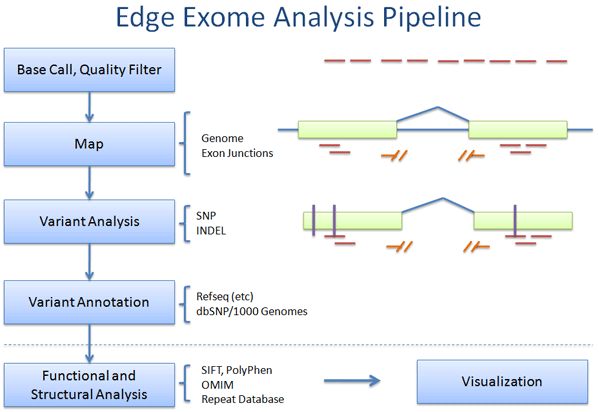
\includegraphics[width=0.9\textwidth]{c2.genomics/exome.bx.01.png}
  \end{figure}
\end{frame}

\begin{frame}
  \frametitle{外显子组测序 | 流程 | 生信}
  \begin{figure}
    \centering
    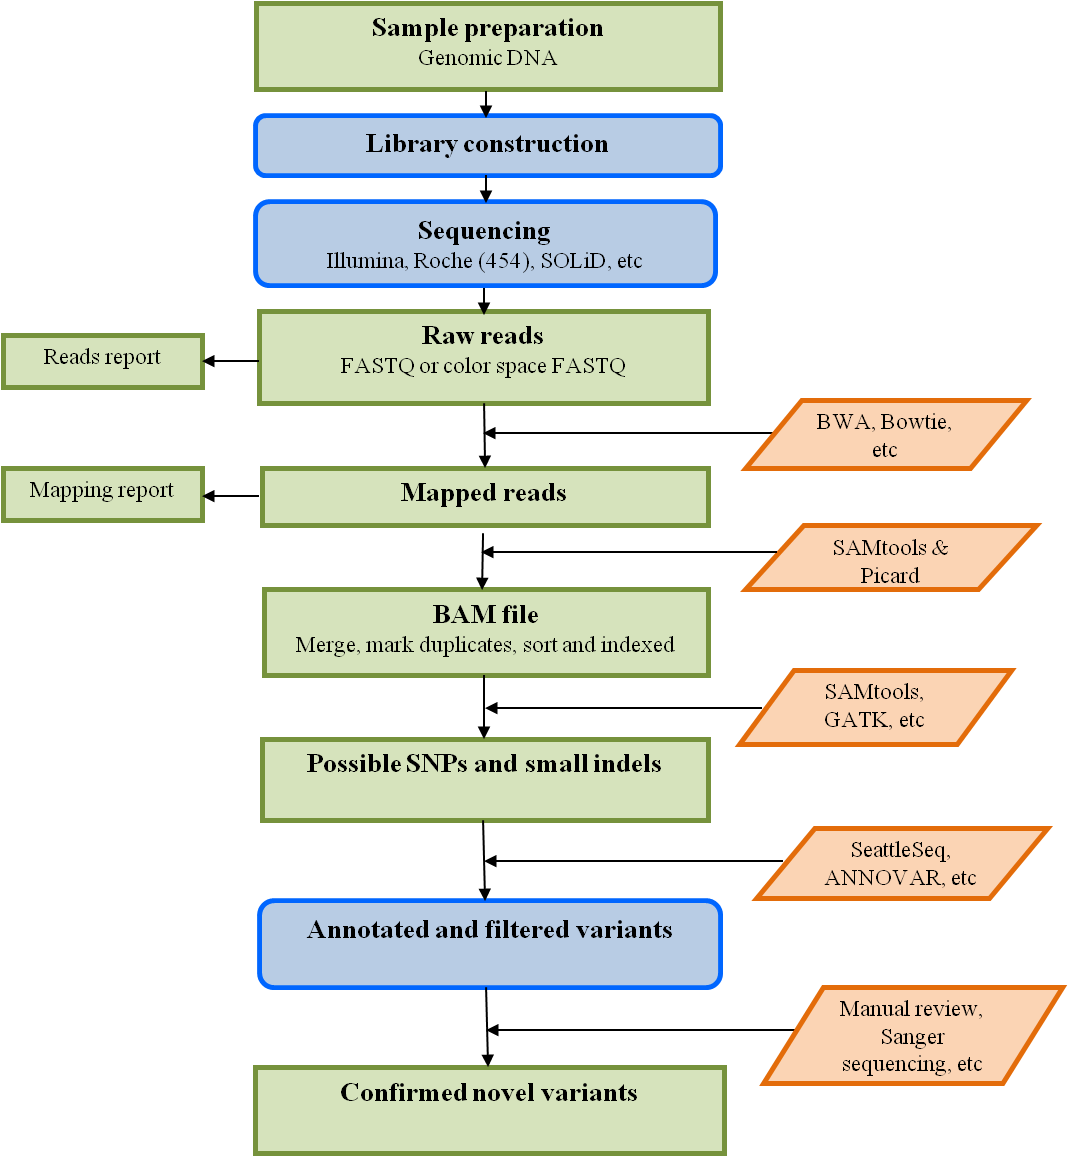
\includegraphics[width=0.6\textwidth]{c2.genomics/exome.bx.03.png}
  \end{figure}
\end{frame}

\begin{frame}
  \frametitle{外显子组测序 | 流程 | 生信}
  \begin{figure}
    \centering
    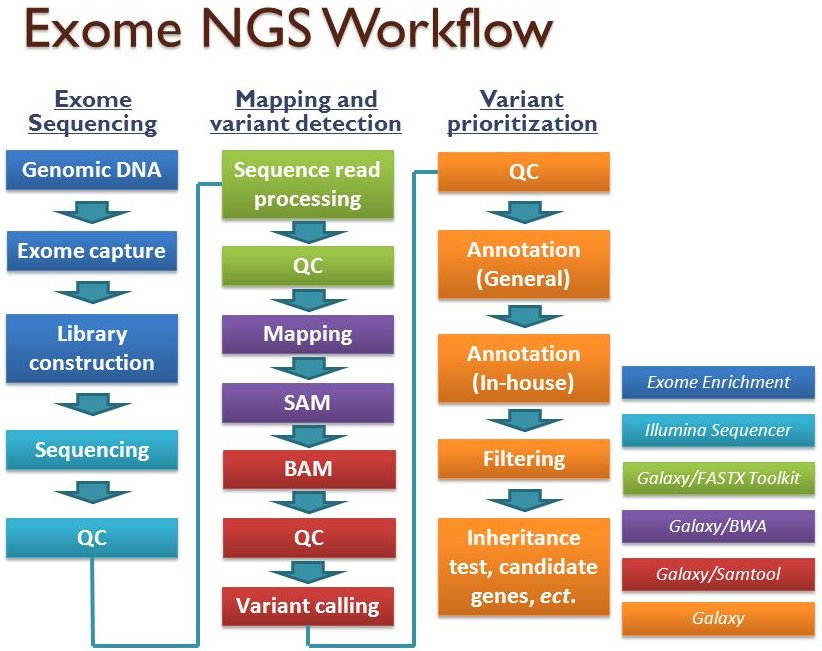
\includegraphics[width=0.8\textwidth]{c2.genomics/exome.bx.04.jpg}
  \end{figure}
\end{frame}

\begin{frame}
  \frametitle{外显子组测序 | 流程 | 生信}
  \begin{figure}
    \centering
    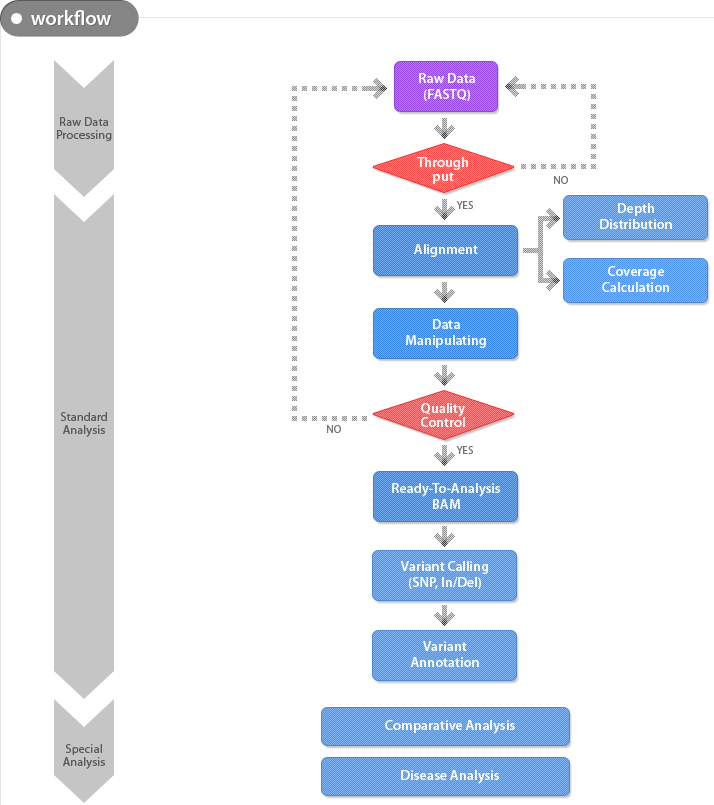
\includegraphics[width=0.55\textwidth]{c2.genomics/exome.bx.02.png}
  \end{figure}
\end{frame}

\begin{frame}
  \frametitle{外显子组测序 | 流程 | 生信}
  \begin{figure}
    \centering
    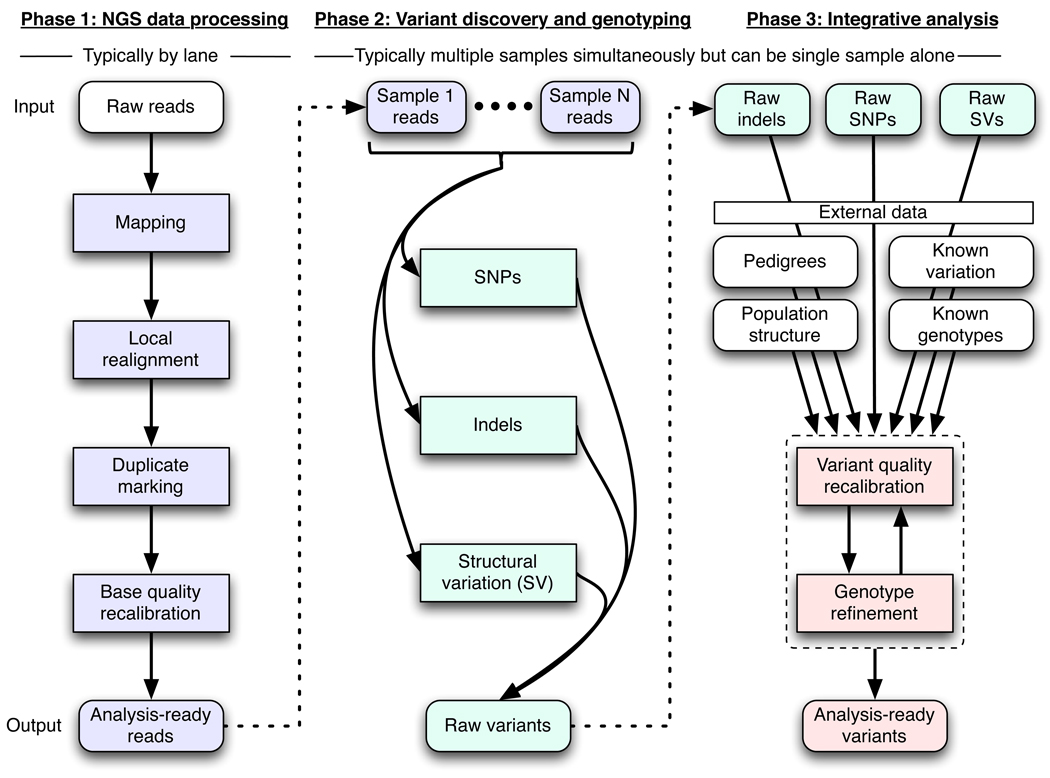
\includegraphics[width=0.9\textwidth]{c2.genomics/exome.bx.07.jpg}
  \end{figure}
\end{frame}

\begin{frame}
  \frametitle{外显子组测序 | 流程 | 生信}
  \begin{figure}
    \centering
    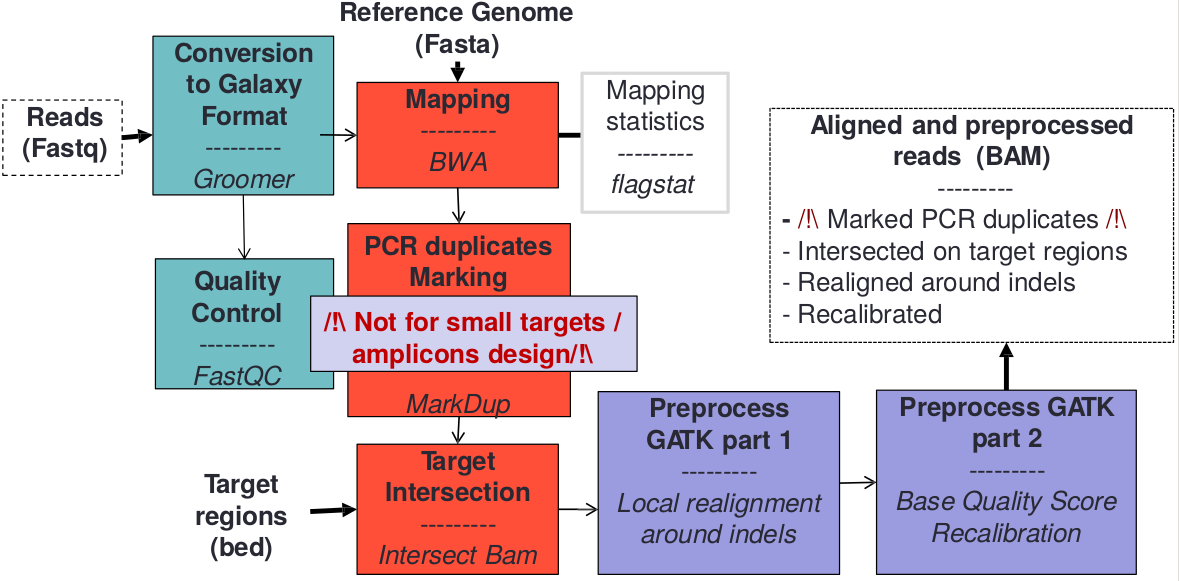
\includegraphics[width=\textwidth]{c2.genomics/exome.bx.08.png}
  \end{figure}
\end{frame}

\begin{frame}
  \frametitle{外显子组测序 | 流程 | 生信}
  \begin{figure}
    \centering
    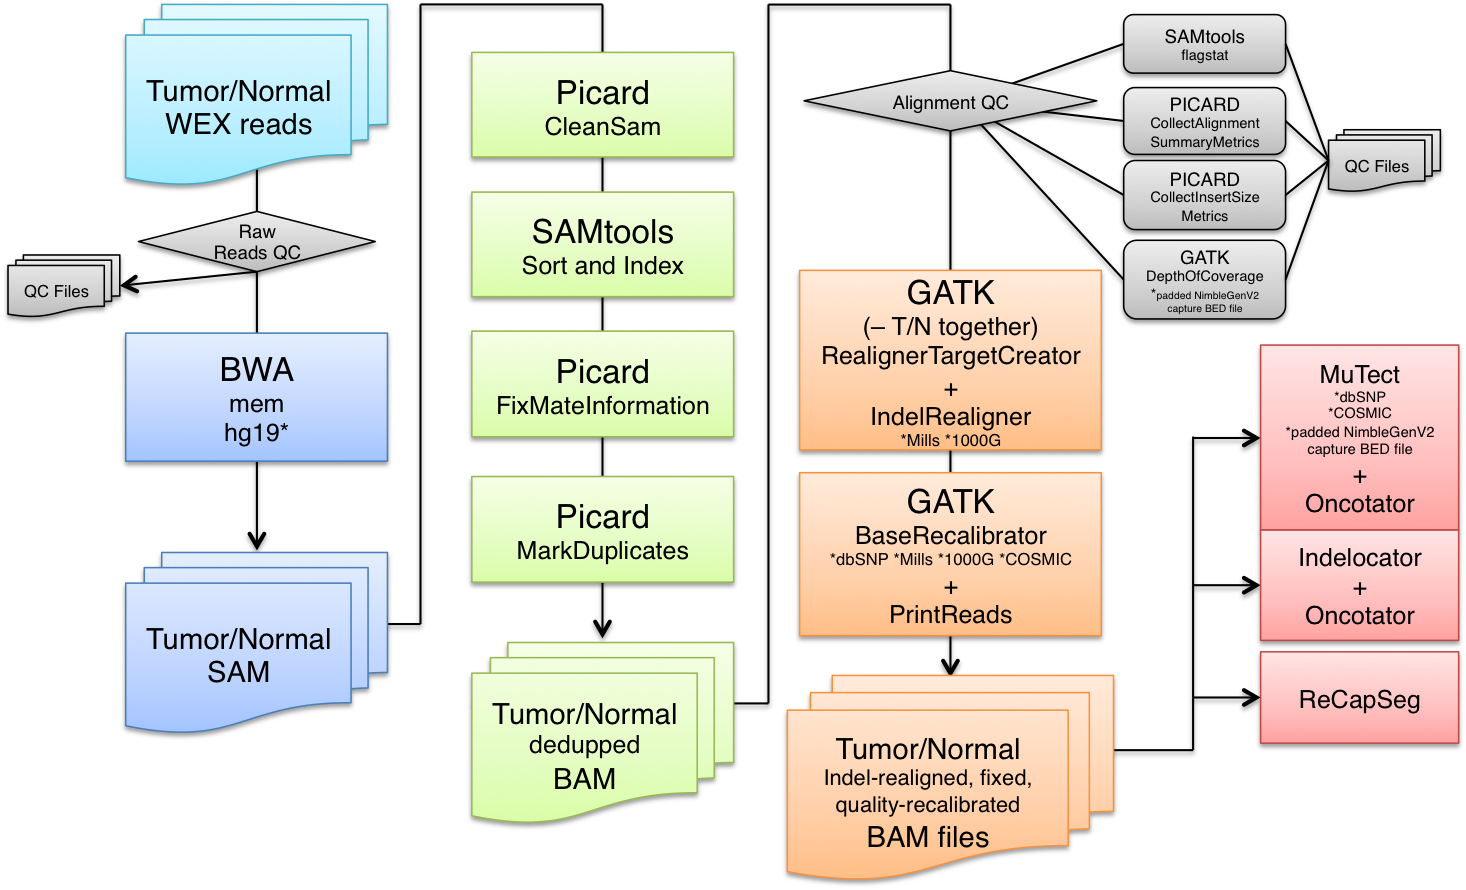
\includegraphics[width=\textwidth]{c2.genomics/exome.bx.05.png}
  \end{figure}
\end{frame}

\begin{frame}
  \frametitle{外显子组测序 | 流程 | 生信}
  \begin{figure}
    \centering
    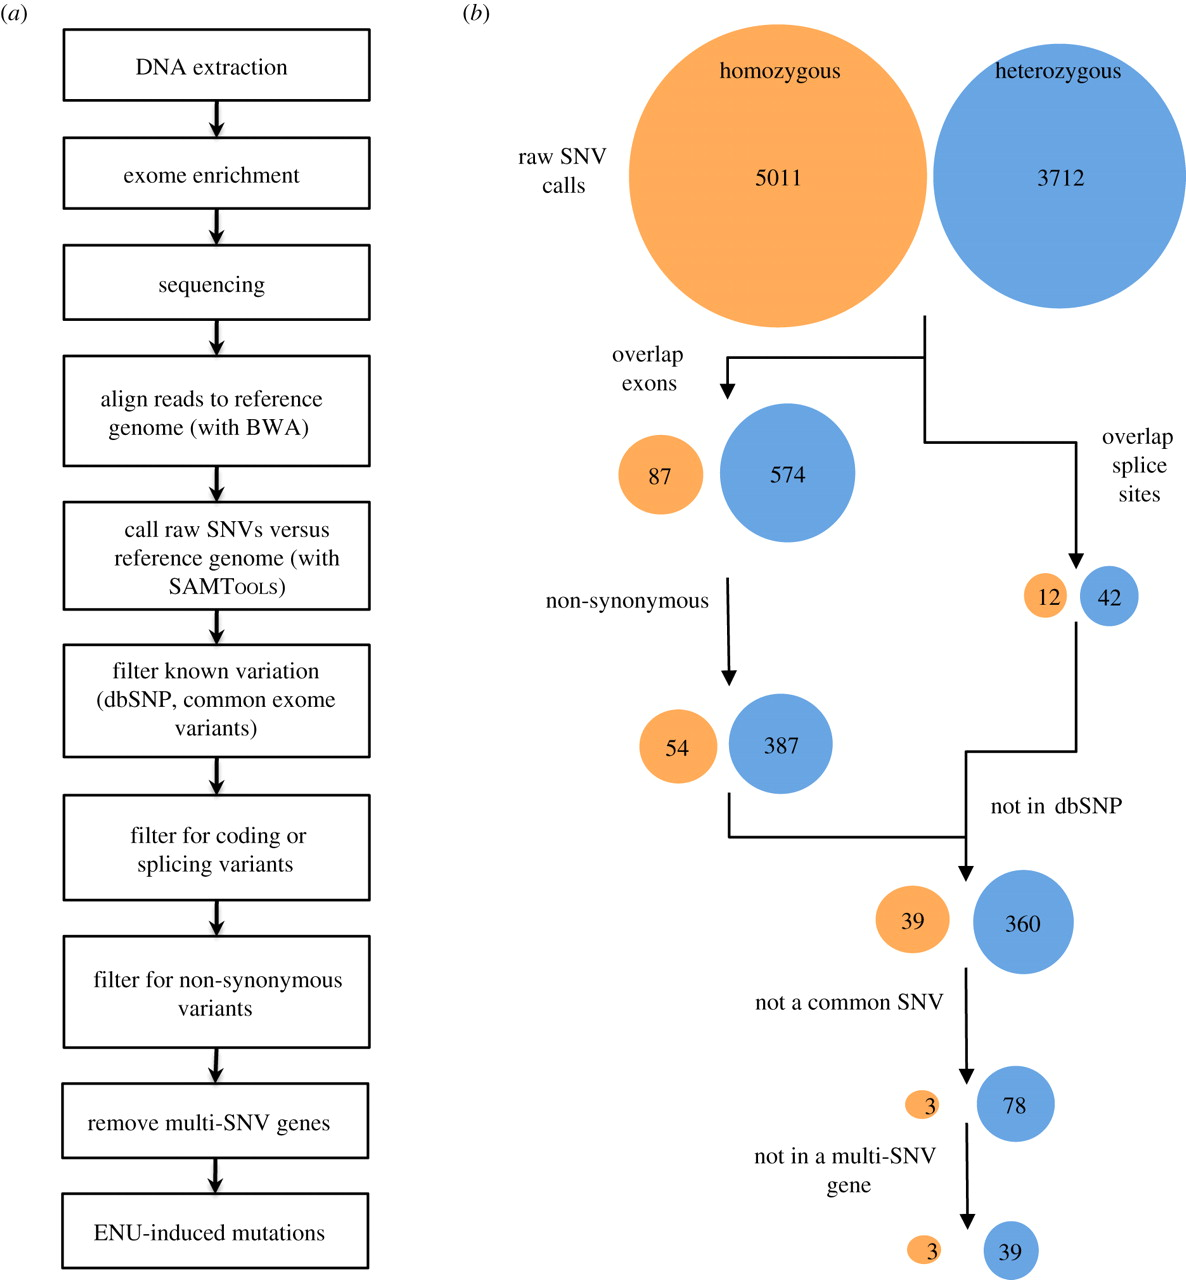
\includegraphics[width=0.6\textwidth]{c2.genomics/exome.bx.06.jpg}
  \end{figure}
\end{frame}

\begin{frame}
  \frametitle{外显子组测序 | 流程 | \textcolor{red}{实验 \& 生信}}
  \begin{figure}
    \centering
    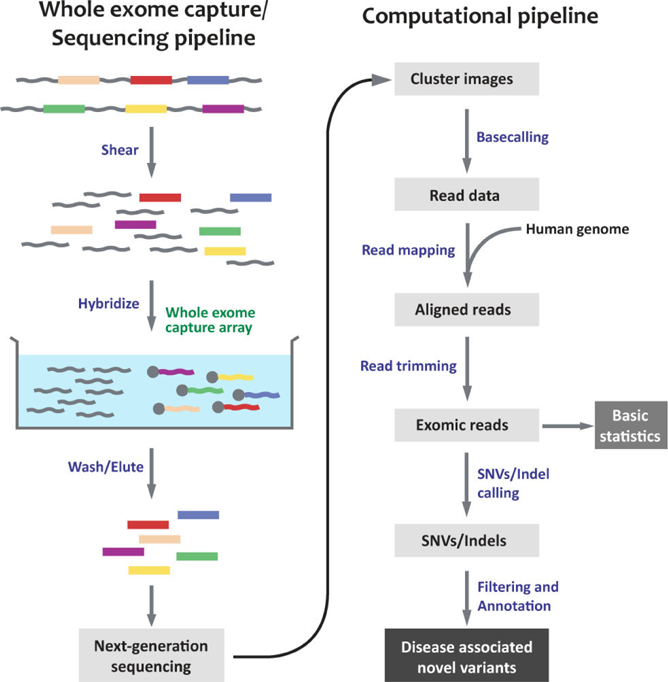
\includegraphics[width=0.6\textwidth]{c2.genomics/exome.exp.bx.01.jpg}
  \end{figure}
\end{frame}

\begin{frame}
  \frametitle{外显子组测序 | 流程 | 实例}
  \begin{figure}
    \centering
    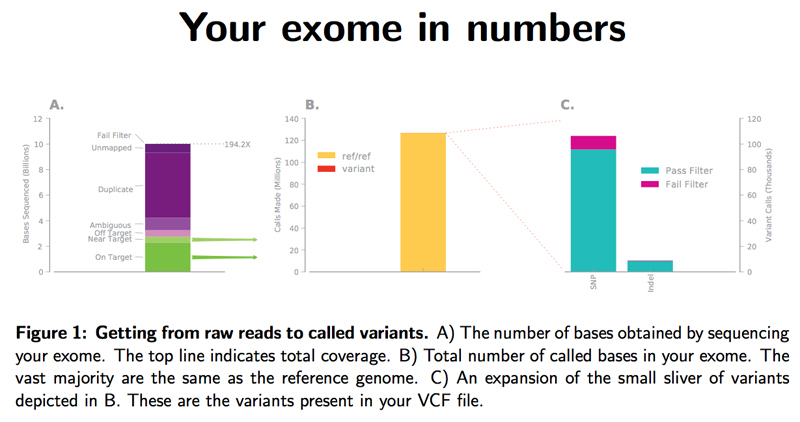
\includegraphics[width=0.9\textwidth]{c2.genomics/exome.case.01.jpg}
  \end{figure}
\end{frame}

\begin{frame}
  \frametitle{外显子组测序 | 流程 | 实例}
  \begin{figure}
    \centering
    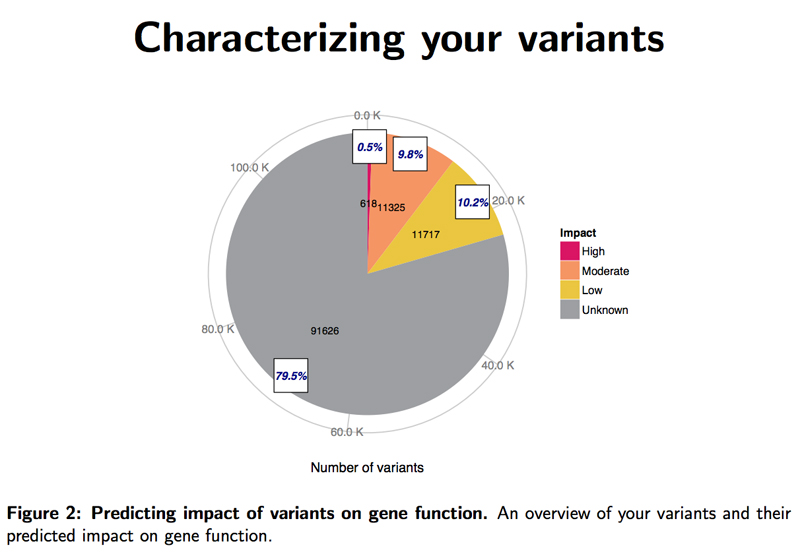
\includegraphics[width=0.9\textwidth]{c2.genomics/exome.case.02.jpg}
  \end{figure}
\end{frame}

\begin{frame}
  \frametitle{外显子组测序 | 流程 | 实例}
  \begin{figure}
    \centering
    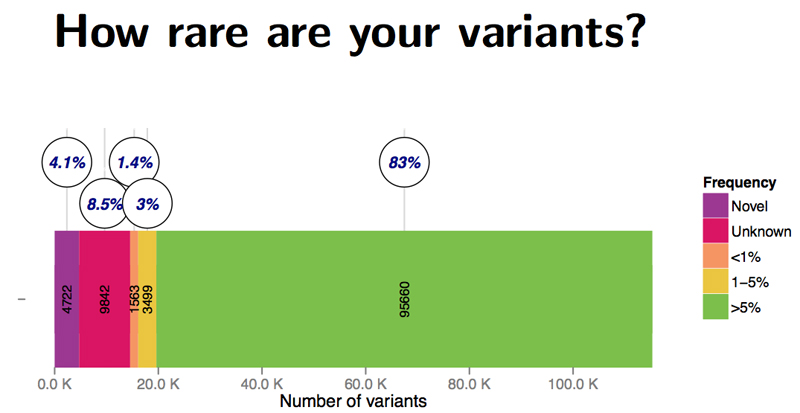
\includegraphics[width=0.9\textwidth]{c2.genomics/exome.case.03.jpg}
  \end{figure}
\end{frame}

\begin{frame}
  \frametitle{外显子组测序 | 流程 | 实例}
  \begin{figure}
    \centering
    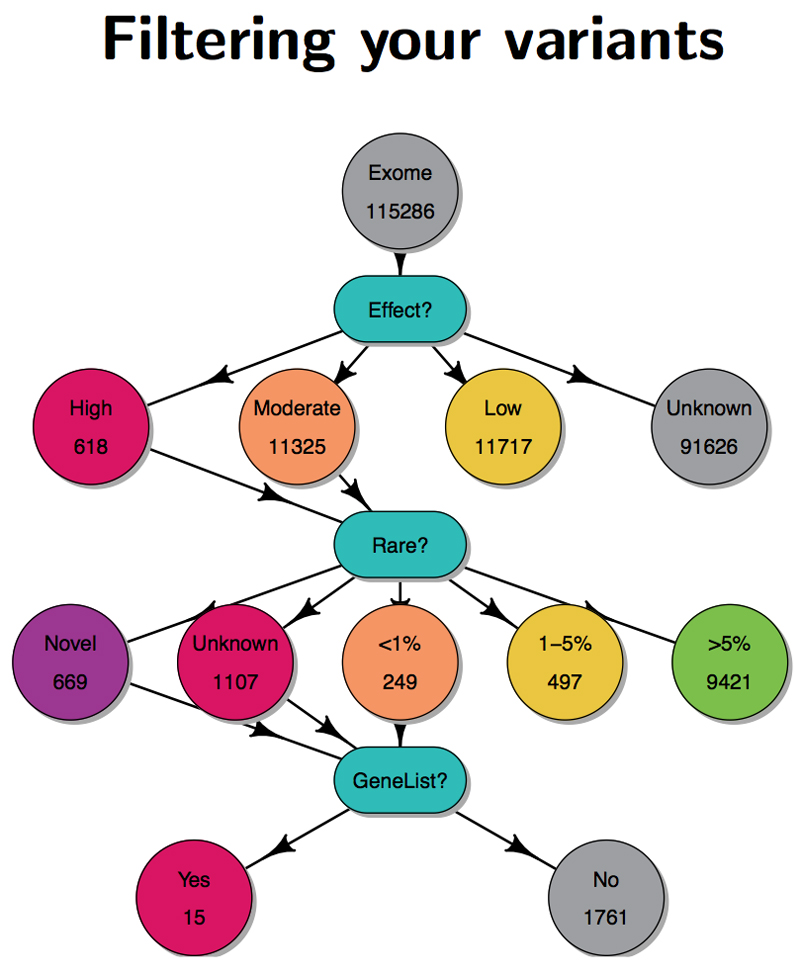
\includegraphics[width=0.5\textwidth]{c2.genomics/exome.case.04.jpg}
  \end{figure}
\end{frame}

\begin{frame}
  \frametitle{外显子组测序 | 流程 | 实例}
  \begin{figure}
    \centering
    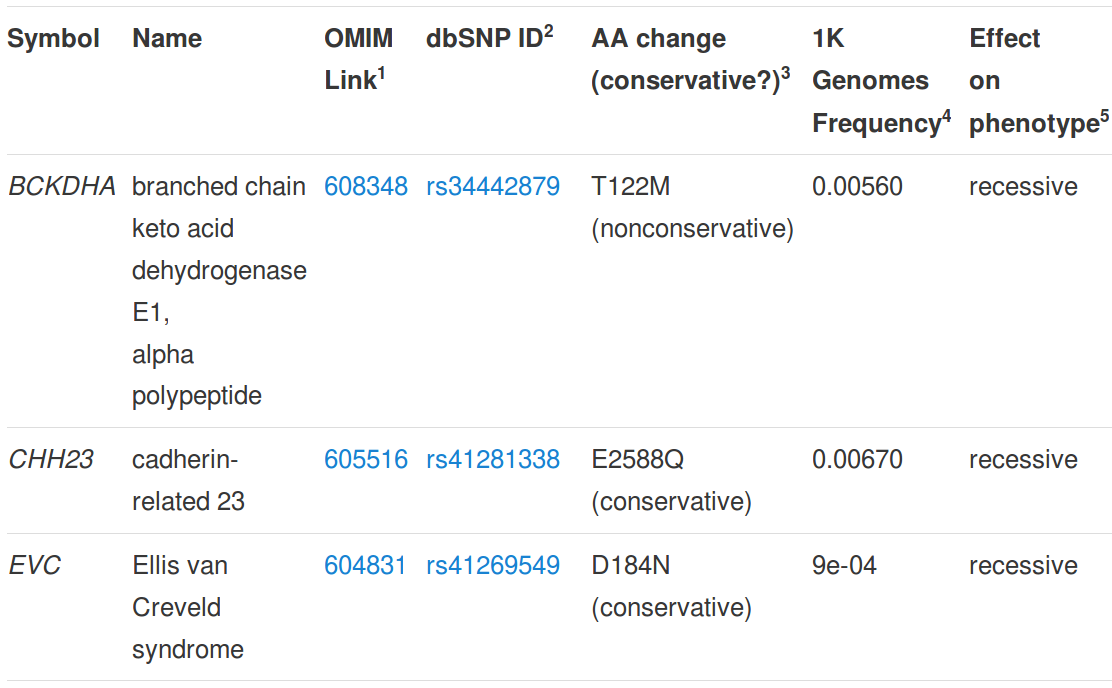
\includegraphics[width=0.9\textwidth]{c2.genomics/exome.case.05.png}
  \end{figure}
\end{frame}

\subsection{应用实例}
\begin{frame}
  \frametitle{基因组学 |  外显子组测序  | 实例}
  A study published in September 2009 discussed a proof of concept experiment to determine if it was possible to identify causal genetic variants using exome sequencing. They sequenced four individuals with Freeman-Sheldon syndrome (FSS) (OMIM 193700), a rare autosomal dominant disorder known to be caused by a mutation in the gene MYH3. Eight HapMap individuals were also sequenced to remove common variants in order to identify the causal gene for FSS. After exclusion of common variants, the authors were able to identify MYH3, which confirms that exome sequencing can be used to identify causal variants of rare disorders. This was the first reported study that used exome sequencing as an approach to identify an unknown causal gene for a rare mendelian disorder.

  Ng SB, Turner EH, Robertson PD, Flygare SD, Bigham AW, Lee C, Shaffer T, Wong M, Bhattacharjee A, Eichler EE, Bamshad M, Nickerson DA, Shendure J (10 September 2009). "Targeted capture and massively parallel sequencing of 12 human exomes". Nature. 461 (7261): 272–276.
\end{frame}

\begin{frame}
  \frametitle{基因组学 | 外显子组测序  | 实例}
  Subsequently, another group reported successful clinical diagnosis of a suspected Bartter syndrome patient of Turkish origin. Bartter syndrome is a renal salt-wasting disease. Exome sequencing revealed an unexpected well-conserved recessive mutation in a gene called SLC26A3 which is associated with congenital chloride diarrhea (CLD). This molecular diagnosis of CLD was confirmed by the referring clinician. This example provided proof of concept of the use of whole-exome sequencing as a clinical tool in evaluation of patients with undiagnosed genetic illnesses. This report is regarded as the first application of next generation sequencing technology for molecular diagnosis of a patient.

  hoi M, Scholl UI, Ji W, Liu T, Tikhonova IR, Zumbo P, Nayir A, Bakkaloğlu A, Ozen S, Sanjad S, Nelson-Williams C, Farhi A, Mane S, Lifton RP (10 November 2009). "Genetic diagnosis by whole exome capture and massively parallel DNA sequencing". Proc Natl Acad Sci U S A. 106 (45): 19096–19101.
\end{frame}

\begin{frame}
  \frametitle{基因组学 | 外显子组测序  | 实例}
  A second report was conducted on exome sequencing of individuals with a mendelian disorder known as Miller syndrome (MIM\#263750), a rare disorder of autosomal recessive inheritance. Two siblings and two unrelated individuals with Miller syndrome were studied. They looked at variants that have the potential to be pathogenic such as non-synonymous mutations, splice acceptor and donor sites and short coding insertions or deletions. Since Miller syndrome is a rare disorder, it is expected that the causal variant has not been previously identified. Previous exome sequencing studies of common single nucleotide polymorphisms (SNPs) in public SNP databases were used to further exclude candidate genes. After exclusion of these genes, the authors found mutations in DHODH that were shared among individuals with Miller syndrome. Each individual with Miller syndrome was a compound heterozygote for the DHODH mutations which were inherited as each parent of an affected individual was found to be a carrier.

  Sarah B Ng; Kati J Buckingham; Choli Lee; Abigail W Bigham; Holly K Tabor; Karin M Dent; Chad D Huff; Paul T Shannon; Ethylin Wang Jabs; Deborah A Nickerson; Jay Shendure; Michael J Bamshad (2010). "Exome sequencing identifies the cause of a mendelian disorder". Nature Genetics. 42 (1): 30–35.
\end{frame}

\begin{frame}
  \frametitle{基因组学 | 外显子组测序  | 实例}
\end{frame}

